%!TEX program = xelatex

\documentclass[print,aspectratio=43]{beamer}
\usepackage[UTF8]{ctex}
\usepackage[english]{babel}

%%%%%%%%%%%%%%%%%%%%%%%%%%%%%%%%%%%%%%%%%%%%%%%%%%%%%%%%%%%%%%%%%%%
% 西文字体:Monaco
% 中文字体:文泉驿微米黑
%%%%%%%%%%%%%%%%%%%%%%%%%%%%%%%%%%%%%%%%%%%%%%%%%%%%%%%%%%%%%%%%%%%
\usepackage{fontspec}
\setmainfont{Monaco}
\setsansfont{Monaco}
\setmonofont{Monaco}
\setCJKmainfont{WenQuanYi Micro Hei}

%%%%%%%%%%%%%%%%%%%%%%%%%%%%%%%%%%%%%%%%%%%%%%%%%%%%%%%%%%%%%%%%%%%
% 添加顔色:solarized light
%%%%%%%%%%%%%%%%%%%%%%%%%%%%%%%%%%%%%%%%%%%%%%%%%%%%%%%%%%%%%%%%%%%
\usepackage{xcolor-solarized}
\usepackage{xcolor}

%%%%%%%%%%%%%%%%%%%%%%%%%%%%%%%%%%%%%%%%%%%%%%%%%%%%%%%%%%%%%%%%%%%
% 代码引用
%%%%%%%%%%%%%%%%%%%%%%%%%%%%%%%%%%%%%%%%%%%%%%%%%%%%%%%%%%%%%%%%%%%
\usepackage{listings}
\lstdefinestyle{base}{
    tabsize=4,
    frame=single, % 单线边框
    frameround=tttt, % 边框圆角,f指尖角,t指圆角,如fttt指一个尖角,三个圆角
    %
    xleftmargin=2em,xrightmargin=2em,aboveskip=1em, % 代码框边界与页面的边距
    %
    % lineskip=-0.05em, % 行距调整
    gobble=2, % 缩进字符数量
    %
    basicstyle=\small\color{black}\fontspec{Monaco},
    keywordstyle=\color{orange!50!black},
    stringstyle=\color{red},
    commentstyle=\color{green!50!black},
    backgroundcolor=\color{solarized-base3},
    %
    breaklines=true,
    showstringspaces=false,
    %
    % numbers=right,
    % numberstyle=\tiny,
}

\lstdefinestyle{sh}{
    style=base,
    language={sh},
}

\lstdefinestyle{rust}{
    style=base,
    language={[GNU]C++},
    morekeywords={in,let,fn},
}

\lstdefinestyle{c}{
    style=base,
    language={[GNU]C++},
}

\lstdefinestyle{go}{
    style=base,
    language={[GNU]C++},
    morekeywords={go,func},
}

\lstset{
    style=sh,
}

%%%%%%%%%%%%%%%%%%%%%%%%%%%%%%%%%%%%%%%%%%%%%%%%%%%%%%%%%%%%%%%%%%%
% 行内代码引用样式
%%%%%%%%%%%%%%%%%%%%%%%%%%%%%%%%%%%%%%%%%%%%%%%%%%%%%%%%%%%%%%%%%%%
\newcommand{\LSTINLINE}[2][sh]{\colorbox{solarized-base3}{\lstinline[style=#1]{#2}}}

\usetheme[navigation]{UMONS}

\newcommand{\en}[1]{\raisebox{-0.16ex}{\,#1\,}}

\title[Git, the king of VCS.]{GIT}
\subtitle{版本控制之王}
\author{范\quad 輝}
\date{\today}
\institute[BeiJing, China]{%
    Rust Engineer\\
    BeiJing, China
    \\[2ex]
    \raisebox{-0.5ex}{
\includegraphics[height=5ex]{figures/logo_git}}
}

\begin{document}
\thispagestyle{empty}
\maketitle

\section{简介}

%%%%%%%%%%%%%%%%%%%%%%%%%%%%%%%%%%%%%%%%%%%%%%%%%%%%%%%%%%%%%%%%%%%%%%%%%%%%%%%%%%%
\subsection{VCS}
%%%%%%%%%%%%%%%%%%%%%%%%%%%%%%%%%%%%%%%%%%%%%%%%%%%%%%%%%%%%%%%%%%%%%%%%%%%%%%%%%%%

\begin{frame}{第一代\en{VCS}}
    \begin{columns}[onlytextwidth]
        \column{.6\textwidth}
        \centering
        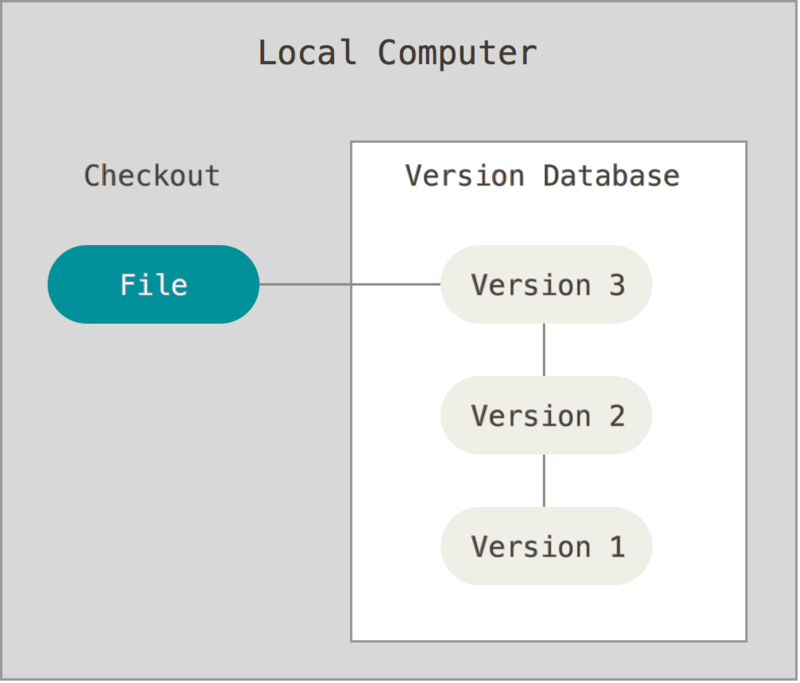
\includegraphics[scale=0.24]{figures/local.png}\\
        \column{.4\textwidth}
        \begin{itemize}
            \item 单点架构
            \item 本地存储
        \end{itemize}
    \end{columns}
\end{frame}

\begin{frame}{第二代\en{VCS}}
    \begin{columns}[onlytextwidth]
        \column{.6\textwidth}
        \centering
        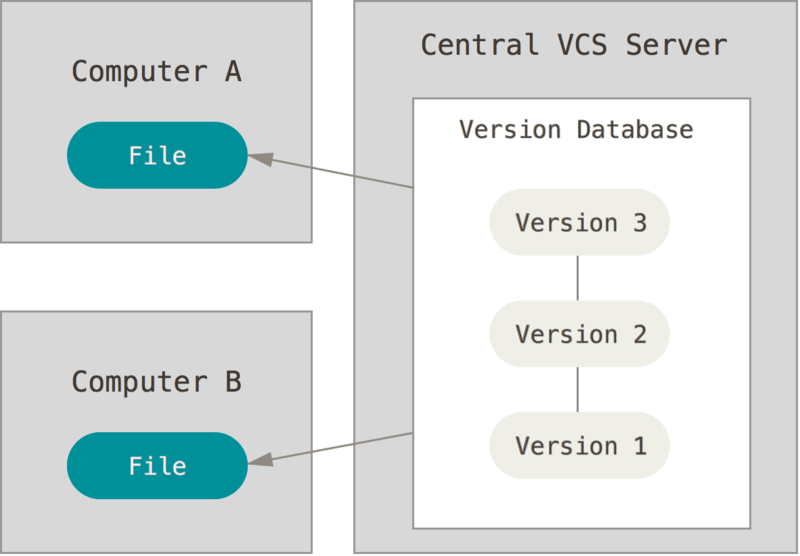
\includegraphics[scale=0.24]{figures/centralized.png}\\
        \column{.4\textwidth}
        \begin{itemize}
            \item \en{C/S}架构
            \item 中心化存储
            \item 典型代表:\en{CVS/Svn}
        \end{itemize}
    \end{columns}
\end{frame}

\begin{frame}{第三代\en{VCS}}
    \begin{columns}[onlytextwidth]
        \column{.6\textwidth}
        \centering
        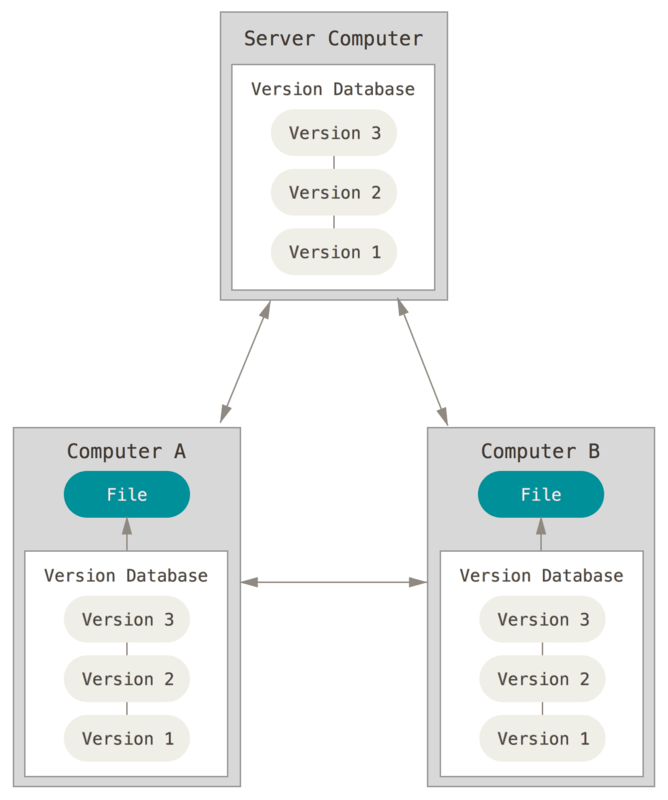
\includegraphics[scale=0.24]{figures/distributed.png}\\
        \column{.4\textwidth}
        \begin{itemize}
            \item \en{P2P}架构
            \item 分布式存储
            \item 典型代表:\en{Git}
        \end{itemize}
    \end{columns}
\end{frame}

%%%%%%%%%%%%%%%%%%%%%%%%%%%%%%%%%%%%%%%%%%%%%%%%%%%%%%%%%%%%%%%%%%%%%%%%%%%%%%%%%%%
\subsection{Git}
%%%%%%%%%%%%%%%%%%%%%%%%%%%%%%%%%%%%%%%%%%%%%%%%%%%%%%%%%%%%%%%%%%%%%%%%%%%%%%%%%%%

\begin{frame}
    \begin{columns}[onlytextwidth]
        \column{.5\textwidth}
        \centering
        
\includegraphics[scale=0.24]{figures/git.png}\\
        \column{.5\textwidth}
        \begin{itemize}
            \item 为自由之信仰而生
            \item 出身名门,天生不凡
            \item 实力碾压一切牛鬼蛇神
        \end{itemize}
    \end{columns}
\end{frame}

\begin{frame}[t]{\en{Git}之父}
    \begin{columns}[onlytextwidth]
        \column{.5\textwidth}
        \begin{exampleblock}{Linus Torvalds}
            \begin{itemize}
                \item \en{Linux}之父
                \item 世界级开源领袖
                \item 人类史上十大黑客之一
            \end{itemize}
        \end{exampleblock}
        \column{.5\textwidth}
        \centering
        
\includegraphics[height=28ex,width=24ex]{figures/linus.jpg}\\
    \end{columns}
\end{frame}

\begin{frame}{\en{Git}的目标}
    \begin{itemize}
        \item Speed
        \item Simple design
        \item Strong support for non-linear development (thousands of parallel branches)
        \item Fully distributed
        \item Able to handle large projects like the Linux kernel efficiently (speed and data size)
    \end{itemize}
\end{frame}

\begin{frame}{\en{Git}的优势}
    \begin{itemize}
        \item 业界最流行方案,主流\en{IDE}默认集成
        \item \href{https://git-scm.com/about/small-and-fast}{运行速度比\en{Svn}快数倍,甚至数百倍}
        \item 分布式架构,支持离线完成绝大多数工作
        \item 极其轻量的本地分支
        \item 便捷的分支合并流程
        \item 强大的数据安全保证
        \item 创新的缓存区设计
        \item 免费且开源
        \item $\cdots$
    \end{itemize}
\end{frame}

\begin{frame}{Git PK Svn}
    \centering
    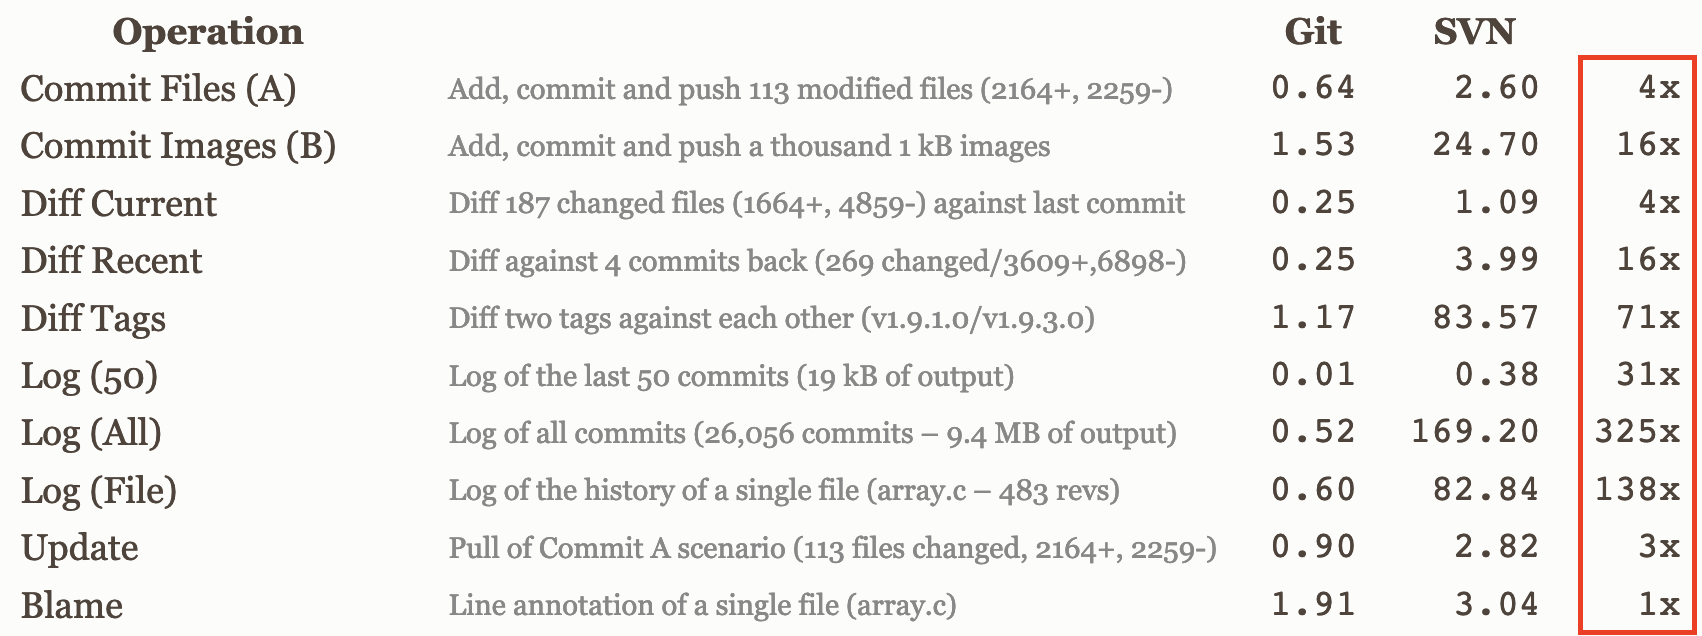
\includegraphics[scale=0.4]{figures/git_vs_svn.png}
\end{frame}

\begin{frame}{\en{Git}的应用场景}
    \begin{itemize}
        \item 版本控制(代码、文档等)
        \item 多人协作
        \item 项目管理(GitHub/GitLab)
        \item 兼容\en{Svn}
        \item CI/CD
        \item $\cdots$
    \end{itemize}
\end{frame}
\section{协作模式}

\begin{frame}{TBD}{Trunk-Based Development}
    \centering
    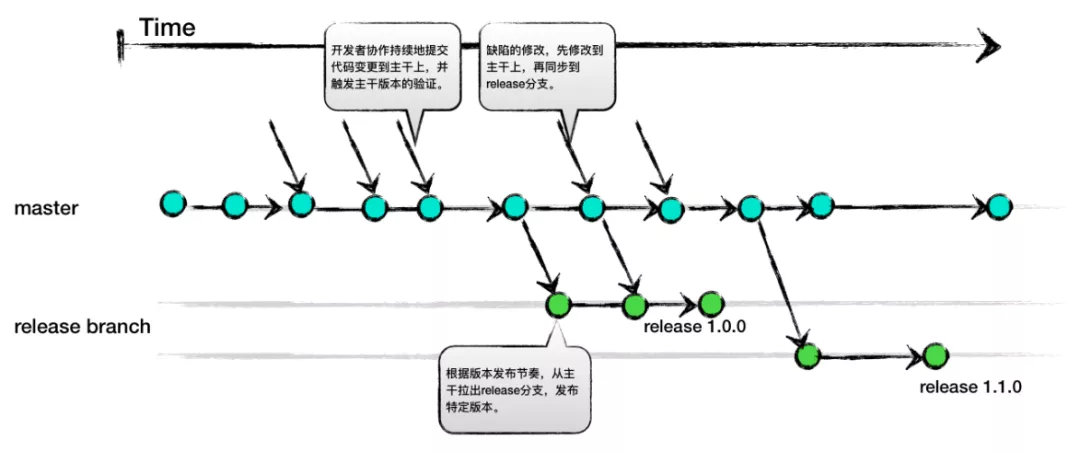
\includegraphics[height=30ex,width=48ex]{figures/tbd.png}
\end{frame}

\begin{frame}[t]{TBD}{优缺点}
    \begin{columns}[onlytextwidth]
        \column{.2\textwidth}
        \column{.6\textwidth}
        \begin{alertblock}{优点}
            \begin{itemize}
                \item 分支少
                \item 操作简单
            \end{itemize}
        \end{alertblock}
        \begin{exampleblock}{缺点}
            \begin{itemize}
                \item 并行开发支持度低
                \item 仅适用于简单版本控制场景
            \end{itemize}
        \end{exampleblock}
        \column{.2\textwidth}
    \end{columns}
\end{frame}

\begin{frame}{Git-Flow}
    \centering
    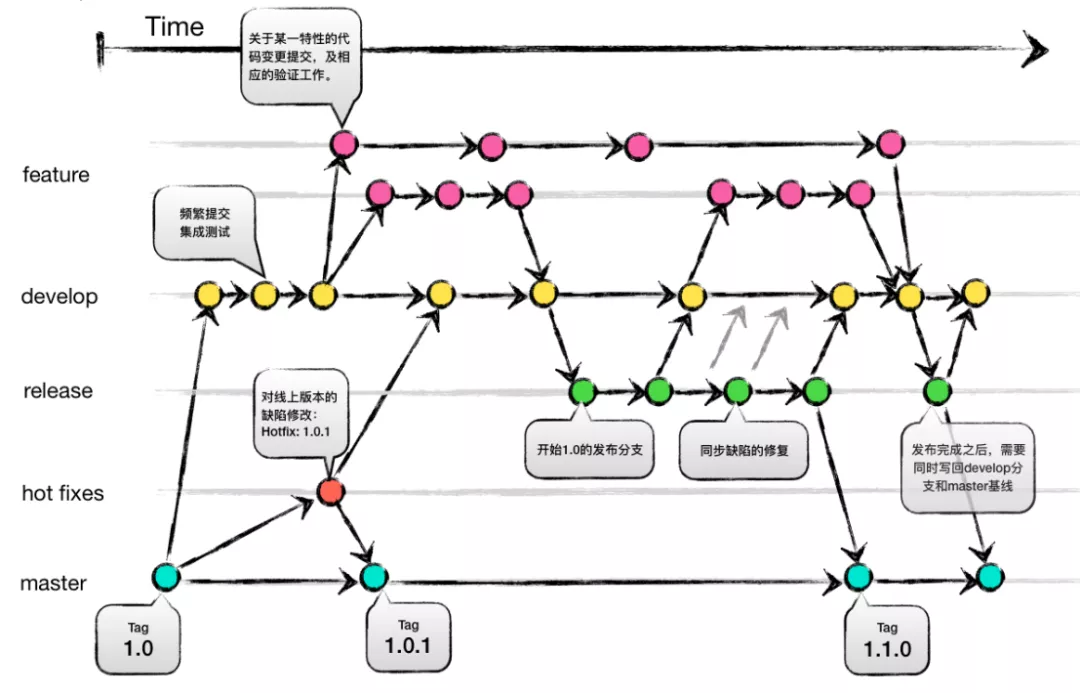
\includegraphics[height=30ex,width=48ex]{figures/git-flow.png}
\end{frame}

\begin{frame}[t]{Git-Flow}{优缺点}
    \begin{columns}[onlytextwidth]
        \column{.2\textwidth}
        \column{.6\textwidth}
        \begin{alertblock}{优点}
            \begin{itemize}
                \item 分支职责清晰
                \item 完善的并行开发支持
                \item 适用于大项目大团队场景
            \end{itemize}
        \end{alertblock}
        \begin{exampleblock}{缺点}
            \begin{itemize}
                \item 分支多
                \item 代码冲突概率大
            \end{itemize}
        \end{exampleblock}
        \column{.2\textwidth}
    \end{columns}
\end{frame}

\begin{frame}{GitHub-Flow}
    \centering
    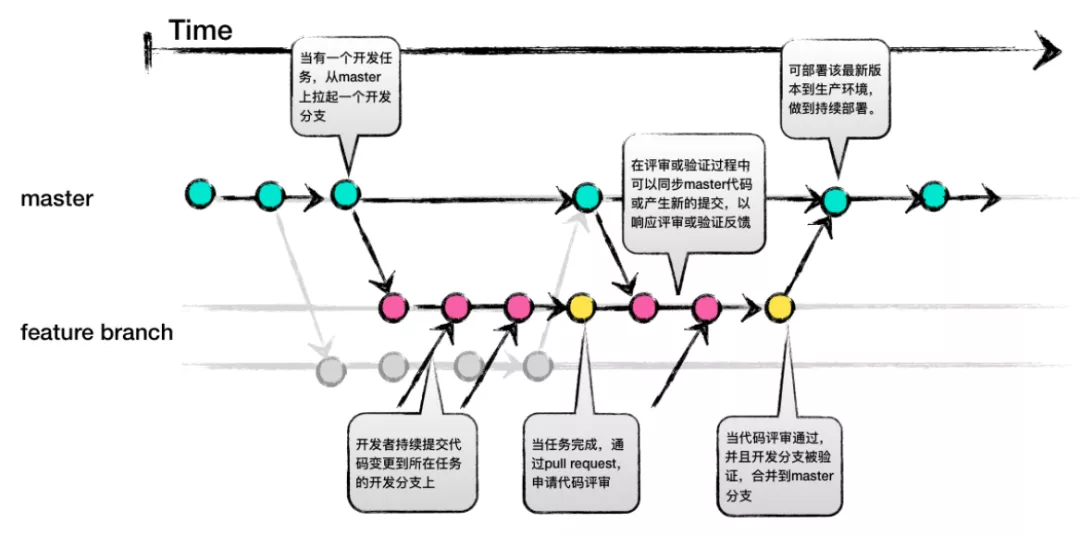
\includegraphics[height=30ex,width=48ex]{figures/github-flow.png}
\end{frame}

\begin{frame}[t]{GitHub-Flow}{优缺点}
    \begin{columns}[onlytextwidth]
        \column{.2\textwidth}
        \column{.6\textwidth}
        \begin{alertblock}{优点}
            \begin{itemize}
                \item 分支逻辑简单
                \item 较高的并行开发支持
                \item 方便与\en{CI/CD}系统集成
            \end{itemize}
        \end{alertblock}
        \begin{exampleblock}{缺点}
            \begin{itemize}
                \item 分支管理不够严谨
            \end{itemize}
        \end{exampleblock}
        \column{.2\textwidth}
    \end{columns}
\end{frame}

\begin{frame}{GitLab-Flow}
    \centering
    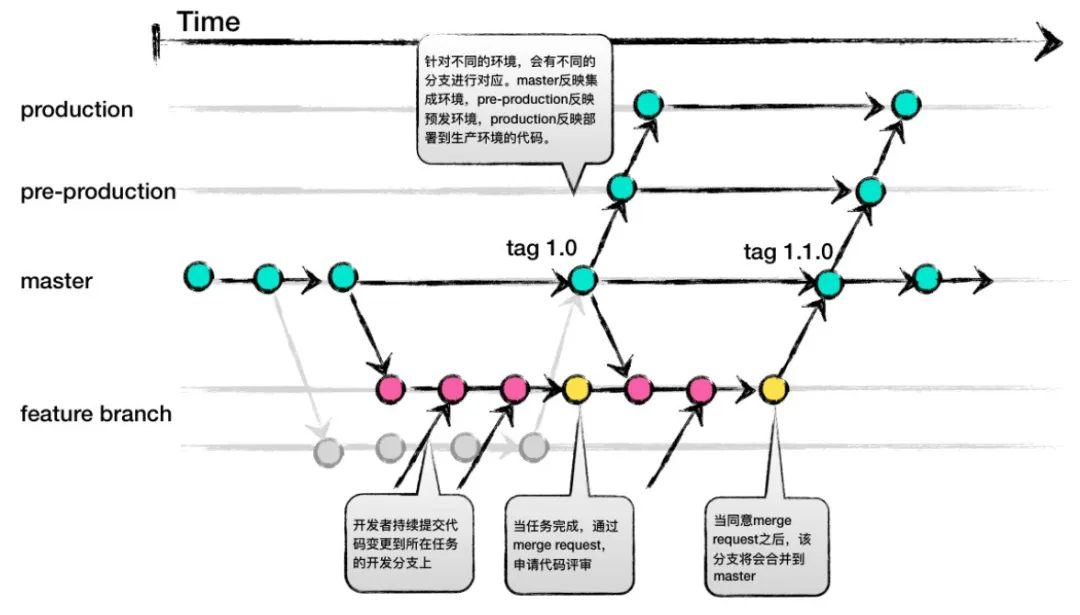
\includegraphics[height=30ex,width=48ex]{figures/gitlab-flow.png}
\end{frame}

\begin{frame}[t]{GitLab-Flow}{优缺点}
    \begin{columns}[onlytextwidth]
        \column{.2\textwidth}
        \column{.6\textwidth}
        \begin{alertblock}{优点}
            \begin{itemize}
                \item 分支管理较严谨
                \item 较高的并行开发支持
                \item 方便与\en{CI/CD}系统集成
            \end{itemize}
        \end{alertblock}
        \begin{exampleblock}{缺点}
            \begin{itemize}
                \item 分支与布署环境过度耦合
                \item 是一种折中方案,复杂度较高
            \end{itemize}
        \end{exampleblock}
        \column{.2\textwidth}
    \end{columns}
\end{frame}
\section{协作平台}

\begin{frame}{总览}
    \begin{description}
        \item[\href{https://gitlab.com}{GitLab}] 提供免费的社区版安装包
        \item[\href{https://github.com}{GitHub}] 世界范围内最知名的\en{Git}协作平台
        \item[\href{https://bitbucket.com}{BitBuck}] 清爽简洁,有一定的用户规模
        \item[\href{https://gitee.com}{GitEE}] 国内最优秀的协作平台,基于\en{GitLab}开发
        \item[\href{https://coding.net}{Coding}] 国内的另一知名协作平台,腾讯系
    \end{description}
\end{frame}

\begin{frame}{GitLab}
    \centering
    
\includegraphics[scale=0.24]{figures/gitlab.png}
\end{frame}

\begin{frame}{GitLab CI/CD (一)}
    \centering
    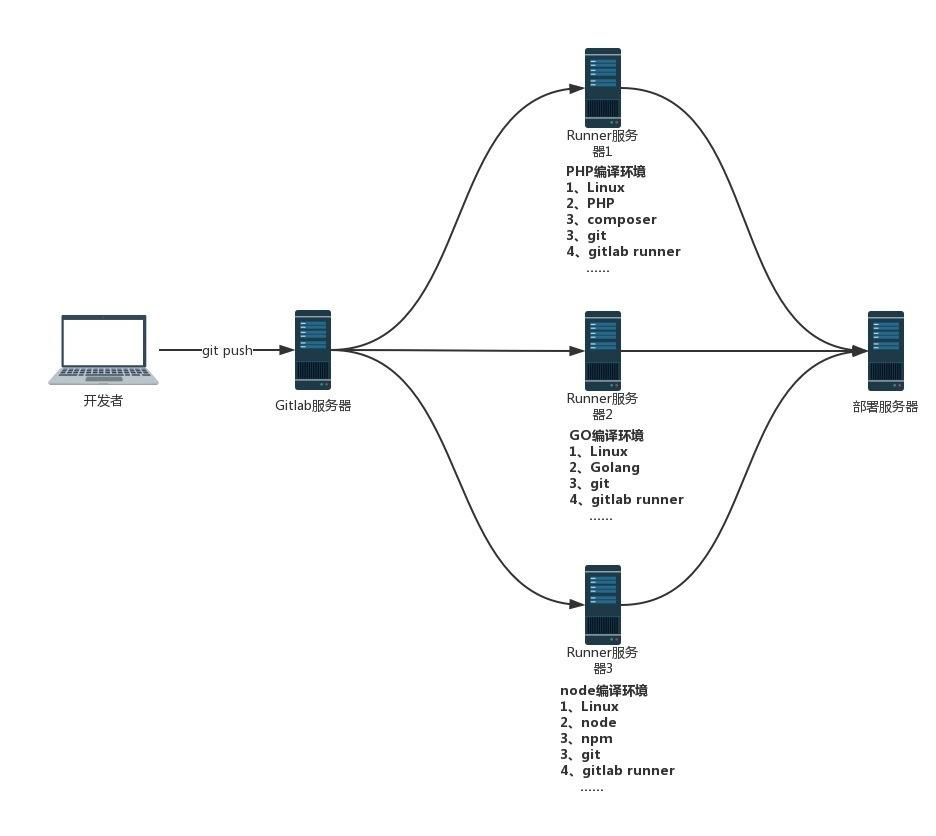
\includegraphics[height=32ex,width=48ex]{figures/gitlab-cicd2.jpg}
\end{frame}

\begin{frame}{GitLab CI/CD (二)}
    \centering
    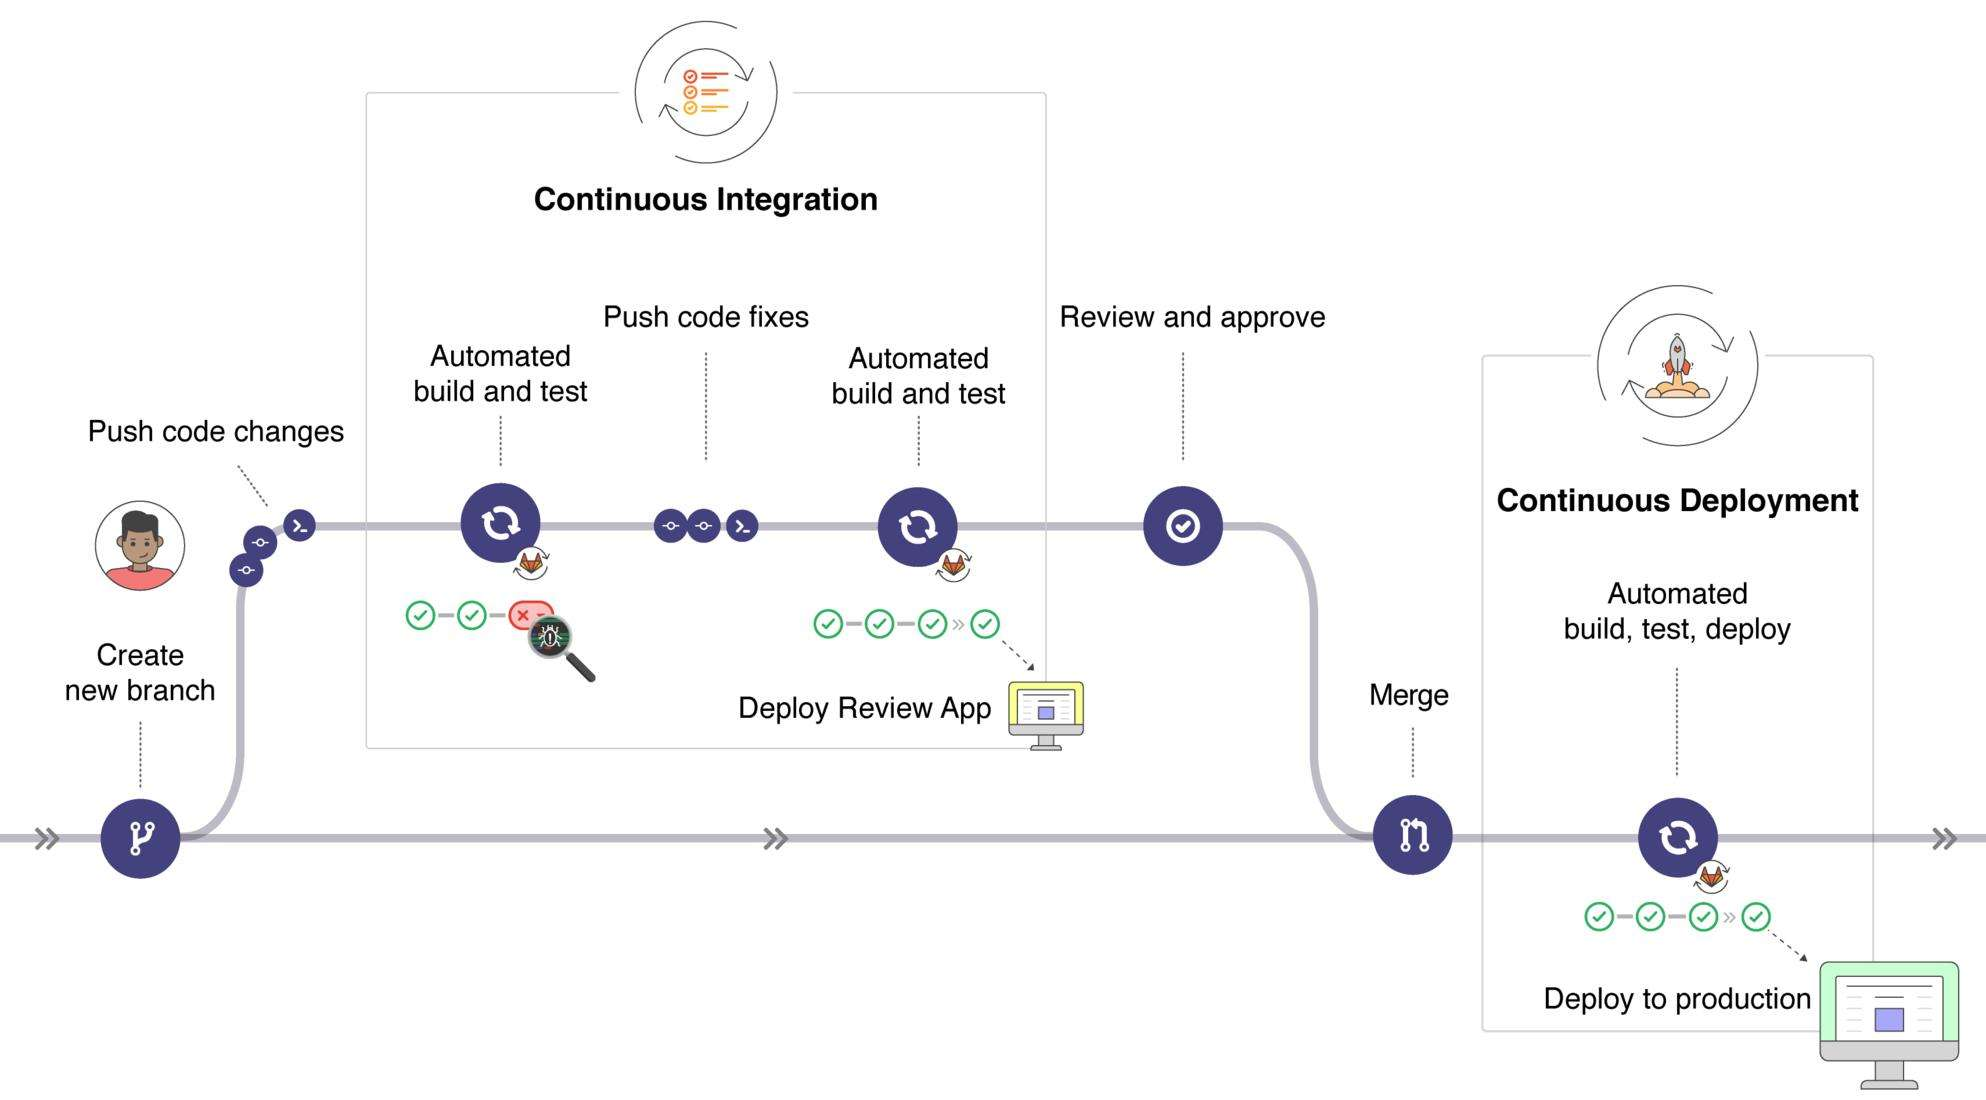
\includegraphics[scale=0.16]{figures/gitlab-cicd.jpg}
\end{frame}

\begin{frame}{GitLab Issue}
    \centering
    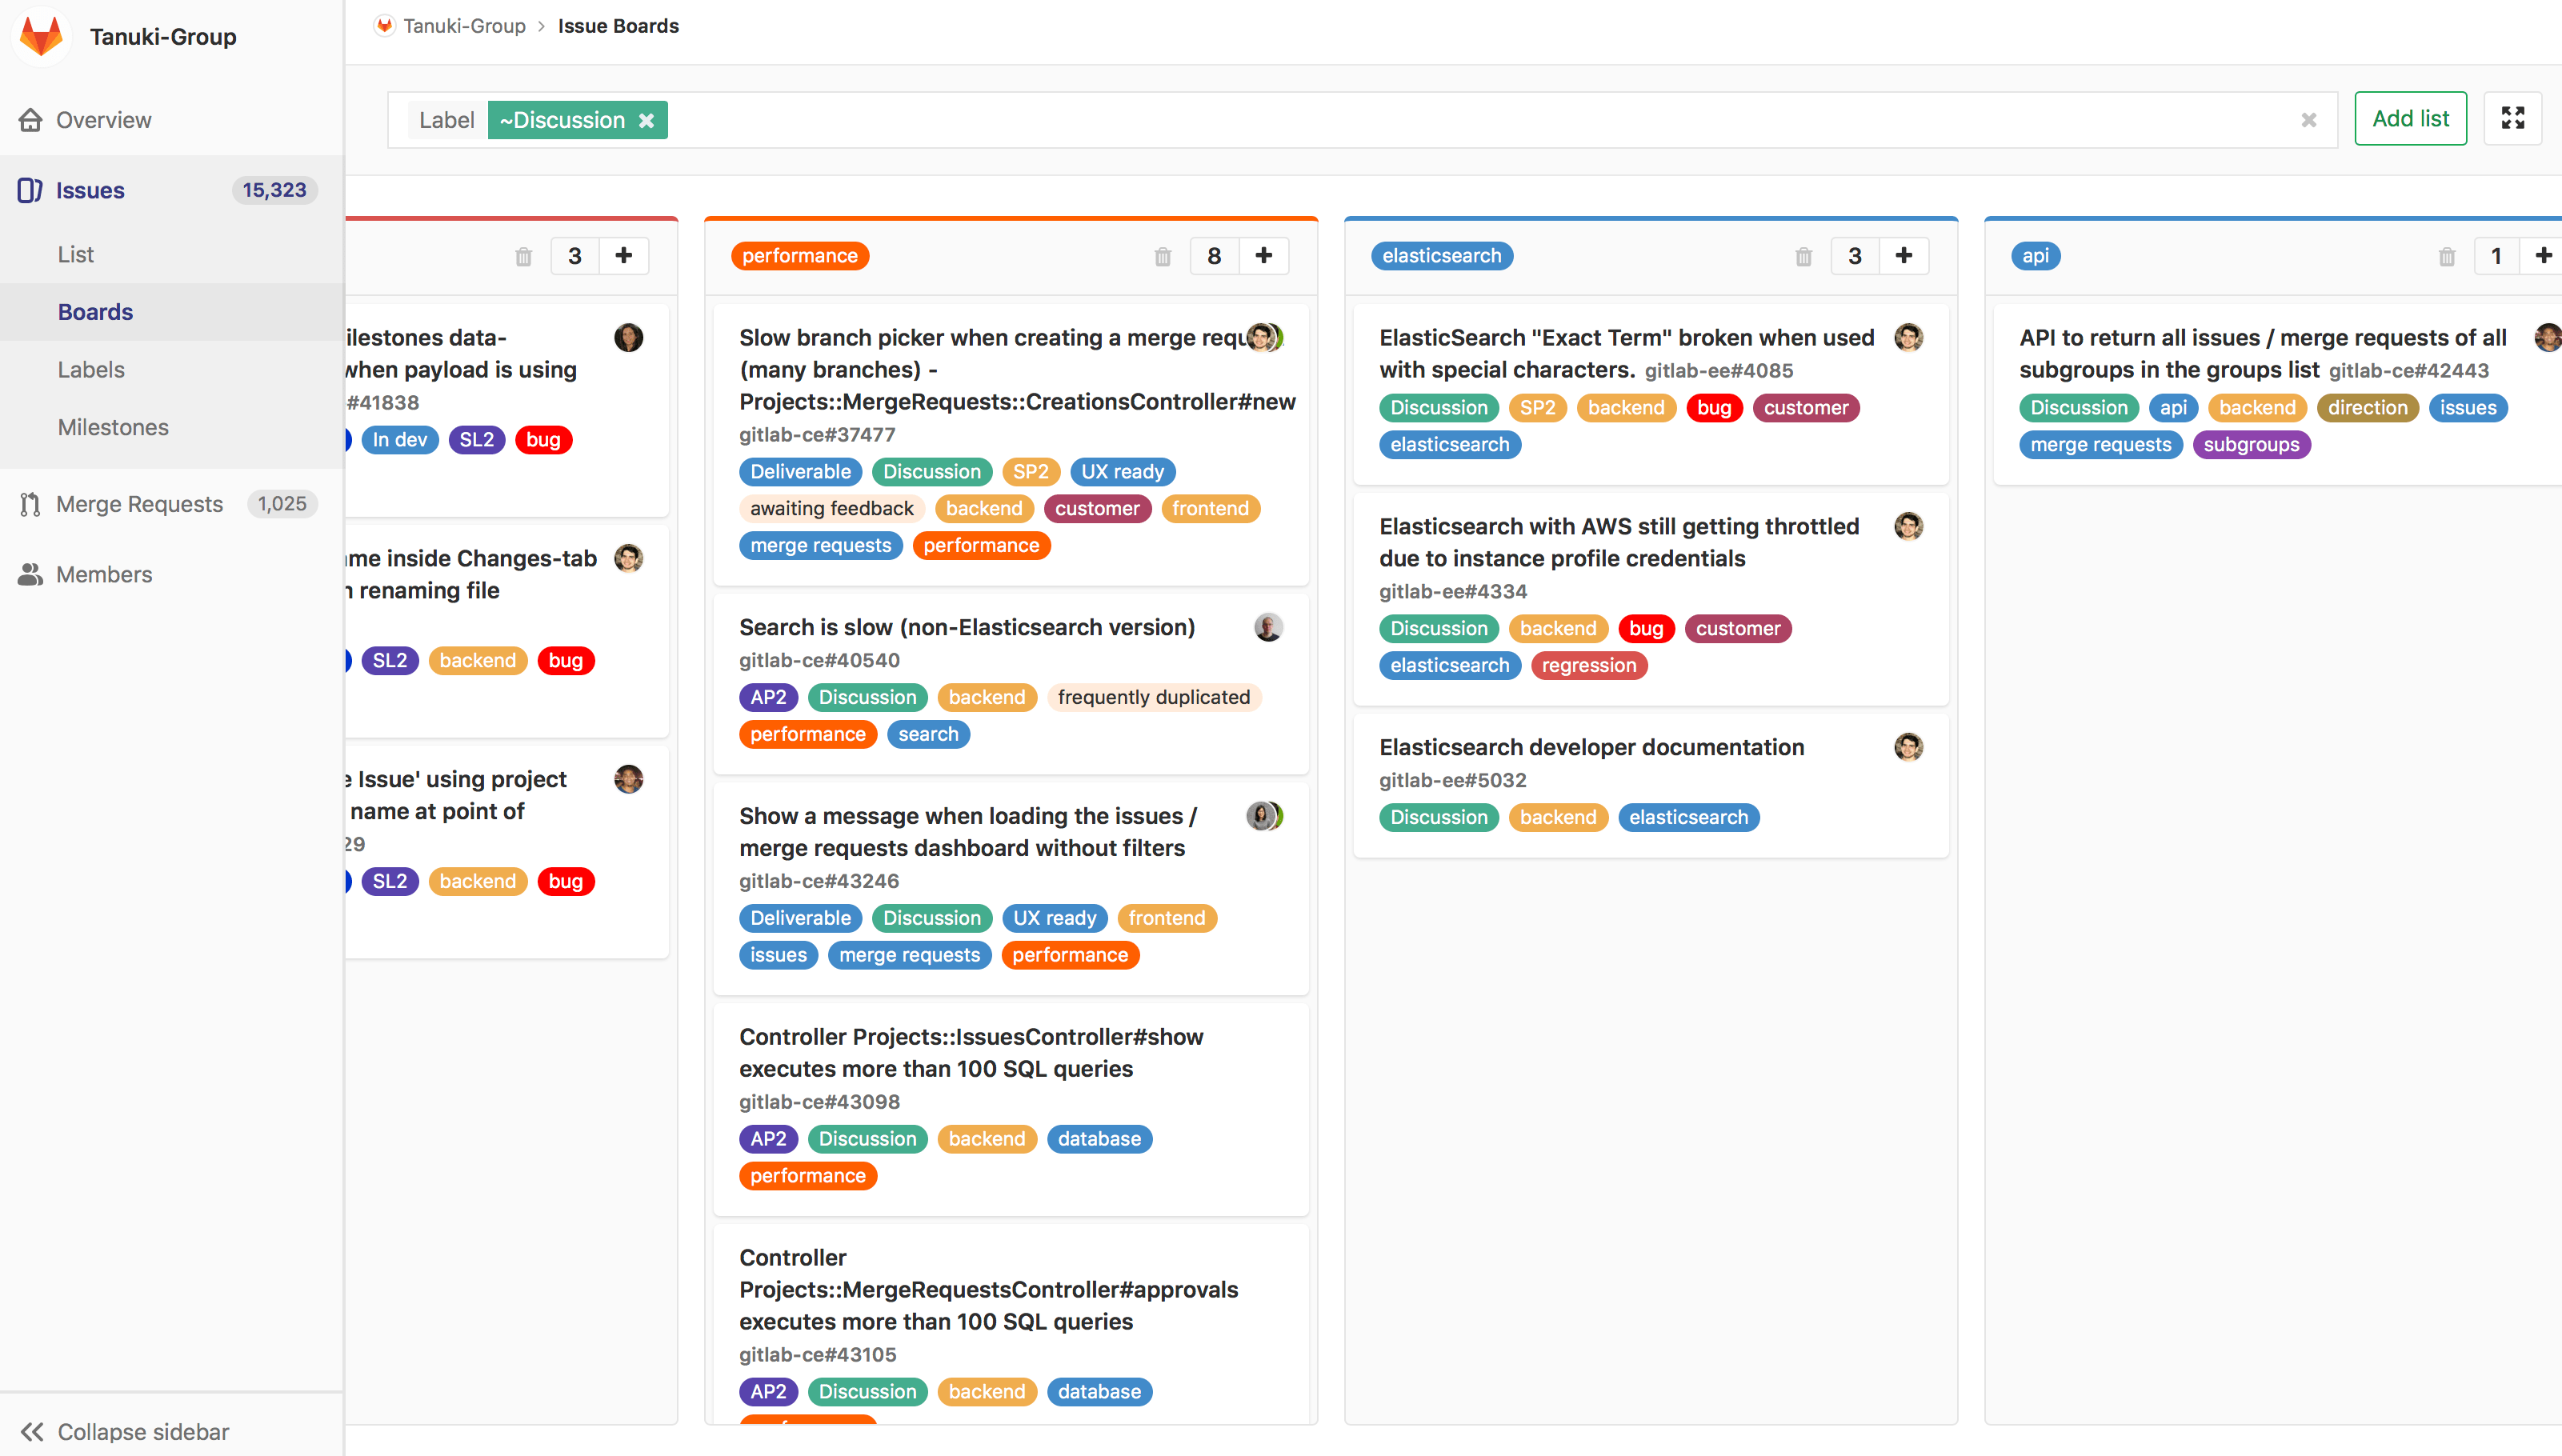
\includegraphics[scale=0.1]{figures/gitlab-issue-dashboard.png}
\end{frame}
\section{命令行}

\begin{frame}[t]{基本操作}
    \centering
    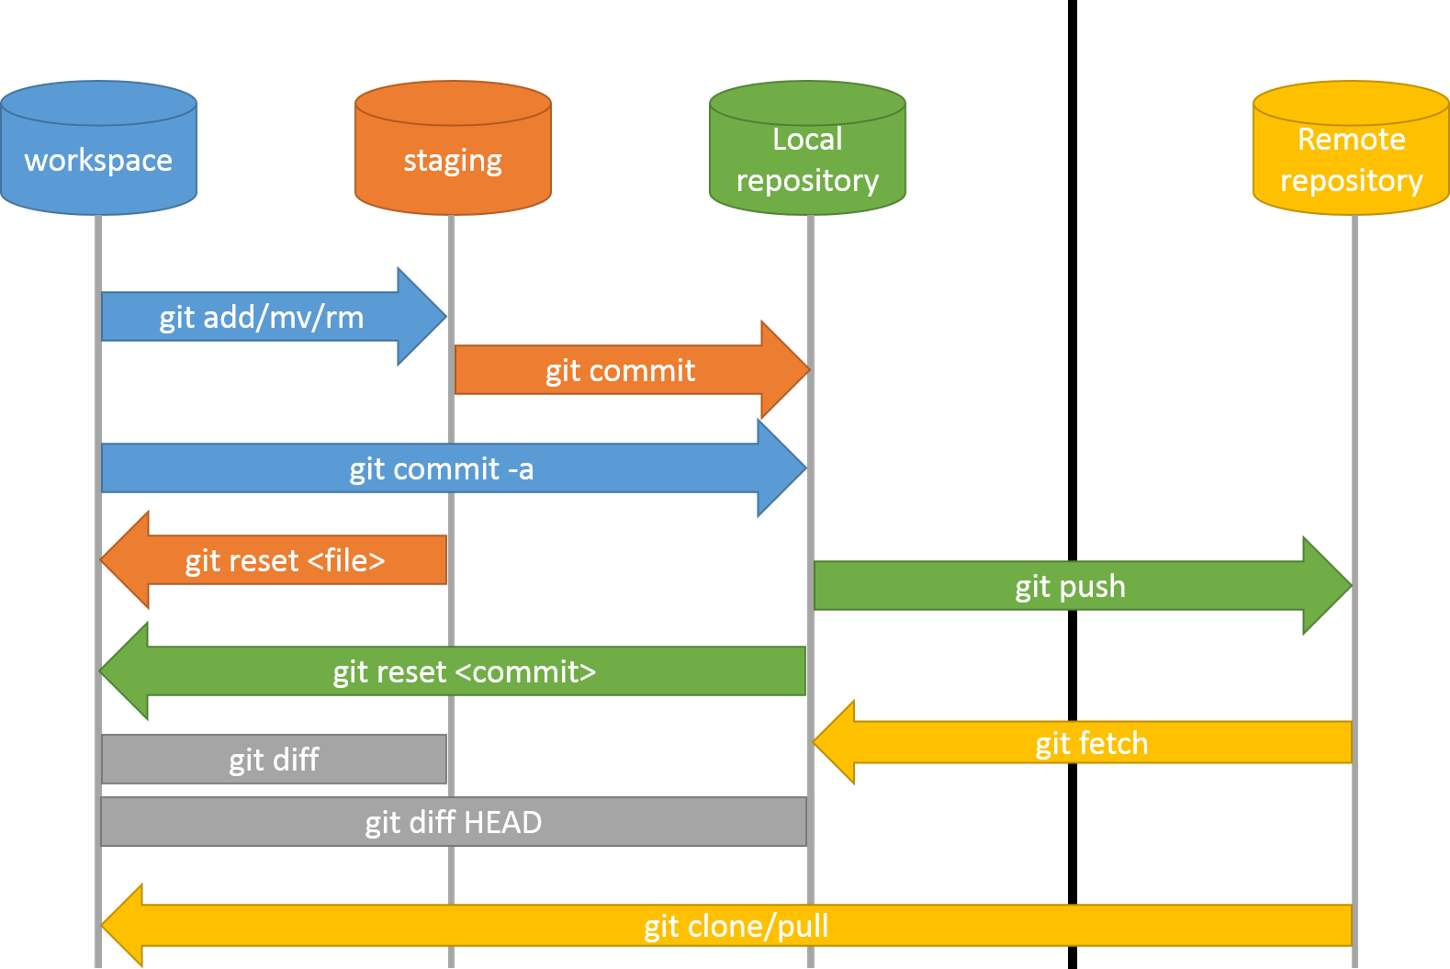
\includegraphics[scale=0.38]{figures/git-basic.jpg}
\end{frame}

\begin{frame}{操作\en{Svn}}
    \centering
    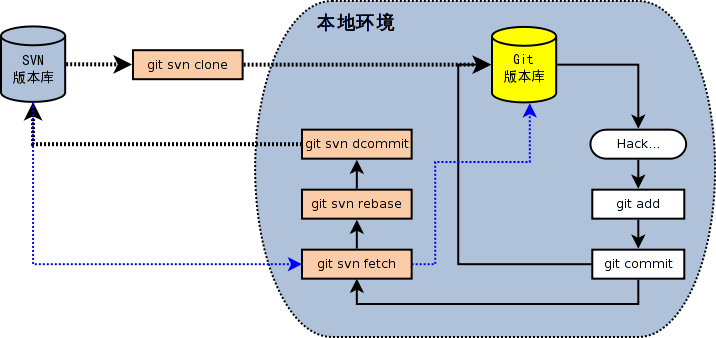
\includegraphics[scale=0.42]{figures/git-svn-basic.jpg}
\end{frame}

\begin{frame}[fragile]{其它常用操作(一)}
    \begin{lstlisting}
        # 查看分支
        git branch -a
        # 切换至指定分支
        git chekcout <BranchName>
        # 基于当前分支创建并切换至新分支
        git checkout -b <BranchName>
        # 合并整个目标分支至当前分支
        git merge --no-ff <BranchName>
        # 合并指定的单次提交至当前分支
        git cherry-pick <CommitID>
        # 删除本地分支
        git branch -D <BranchName>
        # 重命名本地分支
        git branch -m <OldName> <NewName>
    \end{lstlisting}
\end{frame}

\begin{frame}[fragile]{其它常用操作(二)}
    \begin{lstlisting}
        # 添加远程仓库地址
        git remote add <RemoteName> <RemoteAddr>
        # 修改远程仓库地址
        git remote set-url <RemoteName> <RemoteAddr>
        # 删除远程仓库地址
        git remote remove <RemoteName>
        # 删除远程分支
        git push --prune <RemoteName> <RemoteBranch>
        # 创建新标签
        git tag <TagName> <BaseCommitID>
        # 删除标签
        git tag --delete <TagName>
        # 推送本地标签至远程仓库
        git push --tags
    \end{lstlisting}
\end{frame}

\begin{frame}[fragile]{其它常用操作(三)}
    \begin{lstlisting}
        # 基于指定的起点,重新整理提交记录
        git rebase -i <BranchName>
        # 将所有未提交的更改收入隐藏区(垃圾桶)
        git stash
        # 清理所有未纳入版本库管理的文件与目录
        git clean -fdx
        # 查看近期所有分支上的操作日志
        git reflog
        # 查看内容有变动的文件列表
        git diff --name-only <BranchName>
        # 子模块递归更新
        git submodule update --init --recursive
        # 定义指令别名
        git config --global alias.<Alias> <SubCMD>
    \end{lstlisting}
\end{frame}
\section{内部原理}

\begin{frame}[fragile]{数据存储格式(一)}
    \begin{itemize}
        \item 数据存储的核心是一个\en{KV}数据库
        \item 数据单位通过\en{SHA1}散列值进行寻址
        \item 整体结构类似于\en{UNIX}文件系统布局
    \end{itemize}

    \begin{lstlisting}
    $ cd .git/objects && find . -type f

    ./1f/7a7a472abf3dd9643fd615f6da379c4acb3e3a
    ./83/baae61804e65cc73a7201a7252750c76066a30
    ./d6/70460b4b4aece5915caf5c68d12f560a9fe3e4
    \end{lstlisting}
\end{frame}

\begin{frame}{数据存储格式(二)}
    \centering
    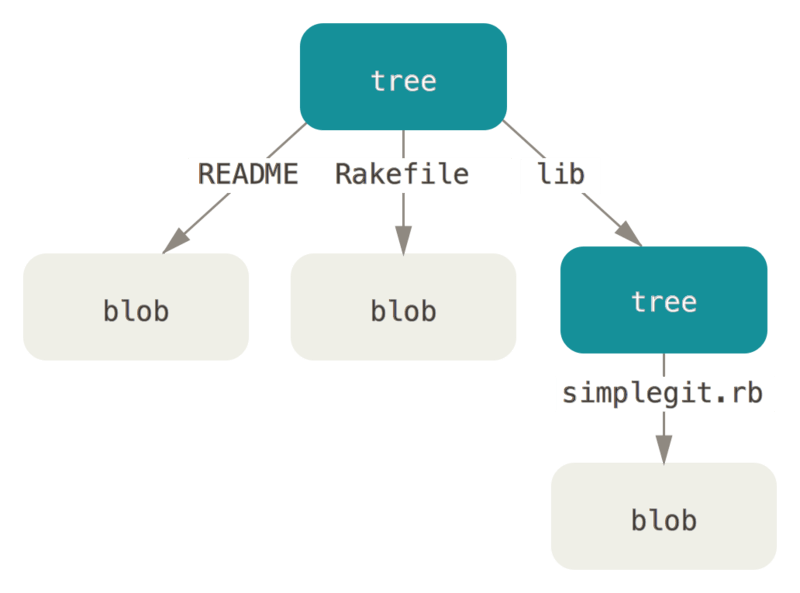
\includegraphics[scale=0.32]{figures/data-model-1.png}
\end{frame}

\begin{frame}{数据存储格式(三)}
    \centering
    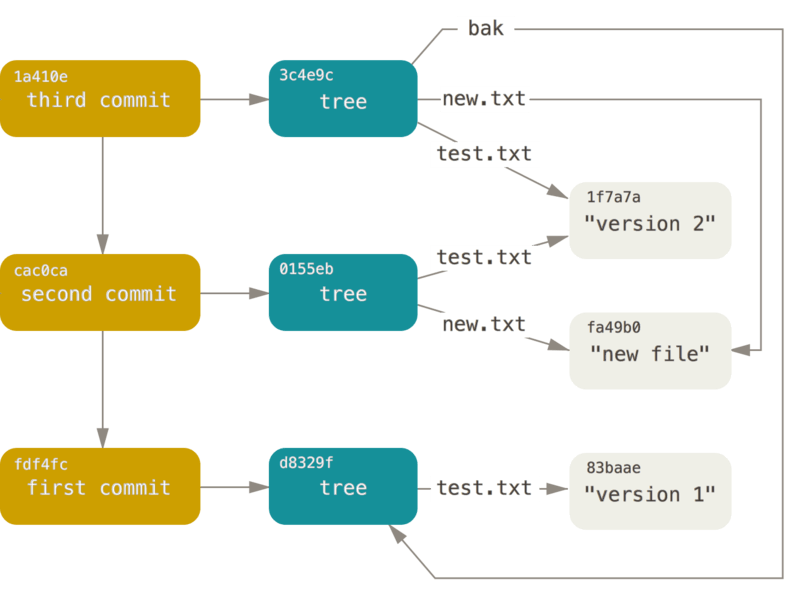
\includegraphics[scale=0.32]{figures/data-model-3.png}
\end{frame}

\begin{frame}{分支与标签的真相}
    \centering
    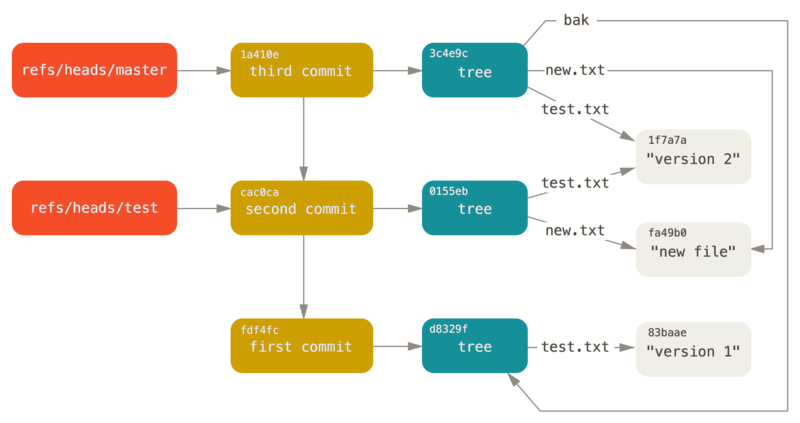
\includegraphics[scale=0.40]{figures/data-model-4.png}
\end{frame}

\section{总结}

\begin{frame}
    \begin{itemize}
        \item 愉悦的团队合作
        \item 巨大的效率提升
    \end{itemize}
    \begin{columns}
    \column{.3\textwidth}
    \rotatebox{15}{\resizebox{128pt}{!}{C\tiny ome}}
    \column{.3\textwidth}
    \rotatebox{15}{\resizebox{128pt}{!}{\raisebox{4pt}{\tiny On}!}}
    \end{columns}
\end{frame}

\begin{frame}{进一步学习}
    \begin{block}{Pro Git}
        \href{https://git-scm.com/book/zh/v2}{https://git-scm.com/book/zh/v2}
    \end{block}

    \begin{block}{\en{Git}源码}
        \href{https://github.com/git/git}{https://github.com/git/git}
    \end{block}

    \begin{block}{\en{Git}第三方开发库}
        \href{https://libgit2.org}{https://libgit2.org}
    \end{block}
\end{frame}

\end{document}